\chapter{Projeto do Sistema Test-Manager}

Este capítulo detalha a concepção estrutural e comportamental do sistema Test-Manager. Nele são apresentados os requisitos funcionais e não funcionais que nortearam o desenvolvimento, bem como os modelos arquiteturais baseados na notação UML, englobando os casos de uso, o diagrama de classes e a modelagem relacional do banco de dados.

\section{Arquitetura do Sistema}

A arquitetura do sistema Test-Manager foi projetada sob o modelo Cliente-Servidor e utiliza o padrão arquitetural Model-View-Controller (MVC), implementado nativamente pelo framework Laravel. Essa estruturação divide as responsabilidades da aplicação em três camadas principais: o Model gerencia a abstração e a persistência dos dados no banco MySQL (utilizando o Eloquent ORM); a View é responsável pela interface com o usuário, construída com os templates Blade e componentes do Bootstrap 5; e o Controller atua interceptando as requisições, aplicando as regras de negócio e coordenando o fluxo de informações entre a interface e o banco de dados.

Para a infraestrutura e execução do projeto, adotou-se a conteinerização por meio da plataforma Docker. Essa ferramenta permite empacotar a aplicação e todas as suas dependências operacionais --- incluindo o servidor web, a linguagem PHP e o banco de dados MySQL --- em contêineres isolados. O uso do Docker garante a padronização do ambiente, eliminando inconsistências entre o desenvolvimento local e o servidor de produção da instituição, além de simplificar e agilizar o processo de implantação (\textit{deploy}) da plataforma.

\section{Requisitos Funcionais}

Os requisitos funcionais representam as operações e os comportamentos essenciais que o sistema deve executar para atender às necessidades de gestão de qualidade de software das equipes do IFES Campus Alegre. O levantamento de dados ocorreu por meio de reuniões com o coordenador e análise do processo atual baseado em planilhas. O Quadro \ref{tab:req_funcionais} apresenta os requisitos mapeados e suas respectivas dependências.

\begin{quadro}[H]
\centering
\caption{Requisitos Funcionais (RF) do Test-Manager.}
\label{tab:req_funcionais}
\small
\begin{tabularx}{\textwidth}{|l|p{3.2cm}|X|l|}
\hline
\textbf{ID} & \textbf{Nome} & \textbf{Descrição} & \textbf{Dependências} \\ \hline
RF01 & Gestão de Acesso & O sistema deve permitir a autenticação segura (login/logout) dos usuários. & - \\ \hline
RF02 & Controle de Papéis & O sistema deve restringir acessos e funcionalidades com base nos perfis: Coordenador, Desenvolvedor e Tester. & RF01 \\ \hline
RF03 & Gestão de Projetos & O Coordenador deve poder criar, listar, editar e remover (CRUD completo) projetos de software. & RF02 \\ \hline
RF04 & Gestão de Usuários & O Coordenador deve poder cadastrar e gerenciar os membros da equipe (Testers e Desenvolvedores). & RF02 \\ \hline
RF05 & Gestão de Casos de Teste & O sistema deve permitir a criação, visualização, edição e exclusão de casos de teste, associando-os a um projeto. & RF03 \\ \hline
RF06 & Importação em Lote & O Coordenador deve ser capaz de importar casos de teste em lote utilizando arquivos estruturados (.csv). & RF05 \\ \hline
RF07 & Versionamento de Testes & O sistema deve gerar versões automáticas (v1.0, v2.0) para os casos de teste, acompanhando o seu ciclo de avaliação. & RF05 \\ \hline
RF08 & Atribuição de Testes & O Coordenador deve ser capaz de atribuir uma versão de um caso de teste a um Tester específico. & RF04, RF07 \\ \hline
RF09 & Execução de Testes & O Tester deve poder registrar a execução de um teste atribuído a ele, marcando-o como `aprovado' ou `reprovado'. & RF08 \\ \hline
RF10 & Registro de Defeitos (Bugs) & Ao reprovar um teste, o sistema deve exigir e registrar os detalhes do defeito encontrado e os passos para reprodução. & RF09 \\ \hline
RF11 & Ciclo de Vida do Defeito & O Desenvolvedor e o Coordenador devem poder atualizar o status de um defeito (Aberto, Em Correção, Resolvido). & RF10 \\ \hline
RF12 & Dashboard e Métricas & O sistema deve apresentar estatísticas em tempo real, como volume de falhas e status dos testes (aprovados/pendentes). & RF01 \\ \hline
RF13 & Rastreabilidade (Logs) & O sistema deve registrar um histórico de auditoria com todas as ações e mudanças de status realizadas nos casos de teste. & RF05 \\ \hline
\end{tabularx}
\fonte{Elaborado pelo autor (2026).}
\end{quadro}

\section{Requisitos Não Funcionais}

Os requisitos não funcionais definem os critérios técnicos de qualidade, usabilidade, segurança e desempenho operacional aos quais a aplicação deve atender. O Quadro \ref{tab:req_naofuncionais} consolida essas premissas.

\begin{quadro}[H]
\centering
\caption{Requisitos Não Funcionais (RNF) do Test-Manager.}
\label{tab:req_naofuncionais}
\small
\begin{tabularx}{\textwidth}{|l|p{3.8cm}|X|}
\hline
\textbf{ID} & \textbf{Nome} & \textbf{Descrição} \\ \hline
RNF01 & Interface e Usabilidade & A interface deve ser responsiva e adaptável a diversos dispositivos (desktops e smartphones), construída com os componentes visuais do framework Bootstrap 5. \\ \hline
RNF02 & Segurança (Autenticação e Roteamento) & As senhas devem ser criptografadas via BCrypt (12 rounds). Todas as rotas administrativas devem ser protegidas por middlewares de autorização por perfil e tokens nativos contra falsificação de solicitações (CSRF). \\ \hline
RNF03 & Desempenho e Paginação & Para garantir a estabilidade e a rapidez na consulta de volumes elevados de casos de teste e defeitos, as listagens devem obrigatoriamente implementar recursos de paginação no servidor. \\ \hline
\end{tabularx}
\fonte{Elaborado pelo autor (2026).}
\end{quadro}

\section{Casos de Uso}

A modelagem de Casos de Uso é essencial para representar as interações comportamentais entre os atores do ecossistema e as funcionalidades disponibilizadas pelo sistema, garantindo que os requisitos elicitados sejam convertidos em fluxos operacionais claros e testáveis.

O Diagrama de Casos de Uso (Figura \ref{fig:casos_uso}) ilustra o escopo funcional da plataforma, organizando os limites de atuação entre três atores principais: \textbf{Coordenador}, \textbf{Tester} e \textbf{Desenvolvedor}. Observa-se no diagrama uma relação de generalização (herança) do ator \textbf{Coordenador} em direção aos atores \textbf{Tester} e \textbf{Desenvolvedor}. Essa estrutura indica que o Coordenador, além de suas atribuições exclusivas de governança --- que abrangem \textit{Cadastrar Coordenador}, \textit{Cadastrar Usuário}, \textit{Cadastrar Projetos}, \textit{Cadastrar Casos de Teste} (incluindo importação em lote via CSV) e \textit{Gerar projeto em PDF} ---, herda as permissões operacionais para inspecionar e interagir com os fluxos de validação e acompanhamento de defeitos de seus projetos.

No escopo do ator \textbf{Tester}, destacam-se os fluxos voltados à bateria de validação de software: \textit{Acessar Caso de Teste}, \textit{Reprovar Caso de Teste} e \textit{Cadastrar Defeitos}. O caso de uso \textit{Acessar Caso de Teste} permite ao avaliador consultar os roteiros de teste e critérios de aceite atribuídos ao seu usuário. A partir dessa consulta, modela-se um relacionamento de extensão (\texttt{<<extend>>}) com o caso de uso \textit{Atualizar status do caso de teste}. Na notação UML, o estereótipo \texttt{<<extend>>} representa um comportamento condicional ou opcional disparado a partir do caso de uso base: o Tester pode apenas consultar os passos e pré-condições do roteiro ou, caso conclua a bateria de verificação com êxito, estender a interação para atualizar o status da versão avaliada.

Adicionalmente, quando a execução prática de um cenário evidencia uma falha no software avaliado, o Tester aciona o caso de uso \textit{Reprovar Caso de Teste}. No fluxo de regras de negócio do Test-Manager, essa reprovação estabelece uma dependência direta com o caso de uso \textit{Cadastrar Defeitos}: para que a reprovação da versão atual seja efetivada (e uma nova versão pendente, como a \texttt{v2.0}, seja gerada automaticamente para reteste futuro), o sistema exige o preenchimento do registro de defeito correspondente, contendo a descrição da anomalia, os passos para reprodução, a severidade e a captura de tela (\textit{print}) opcional.

Por fim, o ator \textbf{Desenvolvedor} interage diretamente com o caso de uso base \textit{Acessar Defeitos}, por meio do qual visualiza a listagem detalhada de falhas vinculadas aos projetos e atribuídas à sua responsabilidade técnica. De maneira análoga ao fluxo de testes, o caso de uso \textit{Atualizar status do defeito} conecta-se a \textit{Acessar Defeitos} mediante uma relação de extensão (\texttt{<<extend>>}). Isso ocorre porque a alteração de status (transicionando o registro de \textit{Aberto} para \textit{Resolvido} após a correção do código-fonte) constitui um fluxo complementar que ocorre sob condição específica durante a inspeção do defeito, gerando automaticamente um registro de rastreabilidade no histórico do caso de teste. O Quadro \ref{tab:casos_uso} sintetiza a descrição de cada caso de uso e sua rastreabilidade frente aos Requisitos Funcionais.

\begin{figure}[H]
    \centering
    \caption{Diagrama de Casos de Uso do sistema Test-Manager.}
    \label{fig:casos_uso}
    \vspace{0.2cm}
    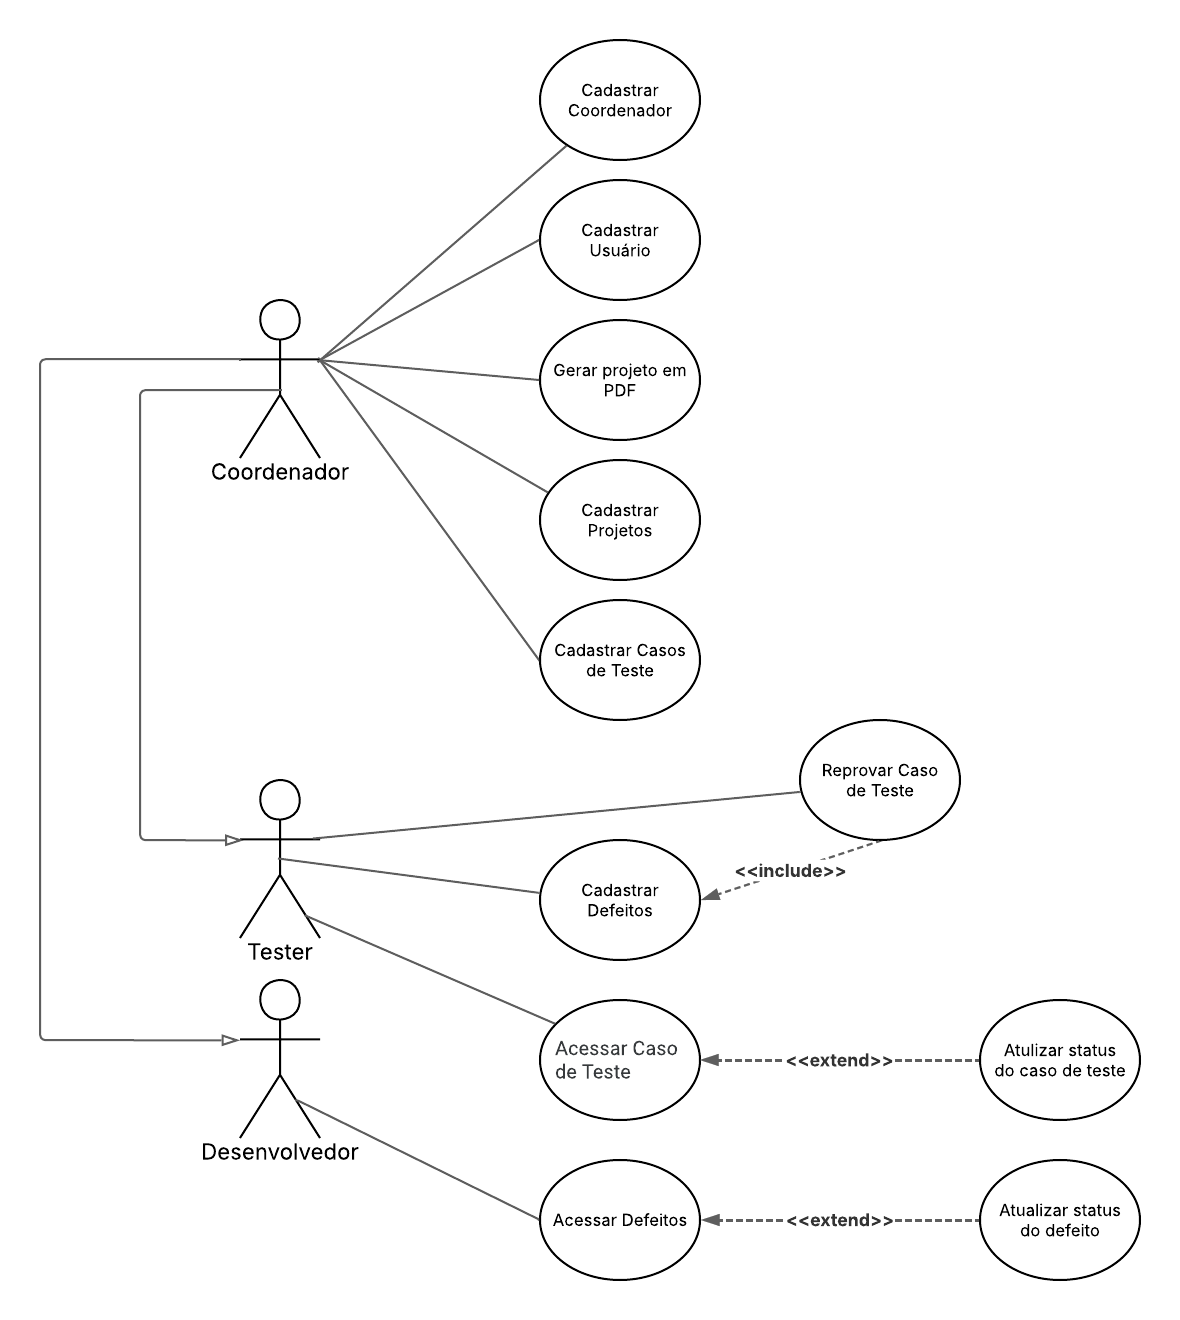
\includegraphics[width=0.88\textwidth, height=0.75\textheight, keepaspectratio]{./figuras/caso_uso_tcc.png} \\
    \vspace{0.2cm}
    {\raggedright \small Fonte: Elaborado pelo autor (2026).\par}
\end{figure}

\clearpage

\begin{quadro}[!htb]
\centering
\caption{Descrição dos Casos de Uso do sistema Test-Manager e sua relação com os Requisitos Funcionais.}
\label{tab:casos_uso}
\footnotesize
\begin{tabularx}{\textwidth}{|l|p{3.2cm}|X|l|}
\hline
\textbf{ID} & \textbf{Caso de Uso} & \textbf{Descrição do Comportamento} & \textbf{Requisitos} \\ \hline
UC01 & Cadastrar Coordenador & O usuário realiza seu próprio cadastro inicial no sistema com o perfil de coordenador. & RF01, RF02 \\ \hline
UC02 & Cadastrar Usuário & O Coordenador cadastra novos Testers e Desenvolvedores, vinculando-os ao ecossistema. & RF02, RF04 \\ \hline
UC03 & Gerar projeto em PDF & O Coordenador gera um relatório consolidado com as informações e métricas do projeto em formato PDF. & RF12, RF13 \\ \hline
UC04 & Cadastrar Projetos & O Coordenador gerencia o registro dos projetos de software da instituição e aloca a equipe. & RF03 \\ \hline
UC05 & Cadastrar Casos de Teste & O Coordenador cria ou importa em lote (.csv) os roteiros de teste e suas versões, associando-os aos projetos. & RF05, RF06, RF07, RF08 \\ \hline
UC06 & Acessar Caso de Teste & O Tester visualiza a lista e os detalhes dos casos de teste e versões atribuídos a ele. & RF05, RF08 \\ \hline
UC07 & Atualizar status do caso de teste & (Extensão de UC06) O Tester altera a situação da versão do teste após realizar sua avaliação prática. & RF09, RF13 \\ \hline
UC08 & Reprovar Caso de Teste & O Tester reprova um cenário de teste cuja execução falhou, iniciando o fluxo de relato da falha e geração de nova versão. & RF07, RF09, RF13 \\ \hline
UC09 & Cadastrar Defeitos & (Dependência de UC08) O Tester ou Coordenador registra os detalhes do bug encontrado, passos de reprodução, severidade e evidência visual. & RF10, RF13 \\ \hline
UC10 & Acessar Defeitos & O Desenvolvedor consulta os defeitos reportados nos projetos e atribuídos à sua responsabilidade. & RF10, RF11 \\ \hline
UC11 & Atualizar status do defeito & (Extensão de UC10) O Desenvolvedor atualiza o status de correção do defeito e gera histórico de auditoria das ações. & RF11, RF13 \\ \hline
\end{tabularx}
\fonte{Elaborado pelo autor (2026).}
\end{quadro}

\section{Modelagem Estrutural}

A modelagem estrutural abstrai a arquitetura interna do sistema, definindo como as informações são representadas no código-fonte por meio de classes e como essas entidades persistem no banco de dados relacional.

\subsection{Diagrama de Classes}

O Diagrama de Classes (Figura \ref{fig:diagrama_classes}) representa a estrutura orientada a objetos da aplicação, mapeando as classes de modelo (\textit{Models}) gerenciadas pelo Eloquent ORM do Laravel, seus atributos encapsulados (visibilidade privada `\texttt{-}'), métodos públicos de negócio e relacionamento (`\texttt{+}') e suas respectivas cardinalidades.

A classe \texttt{User} centraliza o controle de acesso por perfis (\texttt{coordenador}, \texttt{desenvolvedor} e \texttt{tester}) e possui um auto-relacionamento (\texttt{created\_by}) para rastrear qual coordenador cadastrou cada membro da equipe. A classe \texttt{Projeto} armazena o escopo, objetivos e critérios de entrada e saída, associando-se aos usuários de forma muitos-para-muitos por meio da classe associativa \texttt{ProjetoUser} (tabela pivô \texttt{projeto\_user}).

Cada \texttt{Projeto} agrega múltiplos registros de \texttt{CasoDeTeste}, que por sua vez compõem o histórico de auditoria (\texttt{Historico}), os ciclos de execução em \texttt{CasoVersao} (vinculados ao Tester responsável e ao avaliador) e os registros de \texttt{Defeito} (que conectam a falha encontrada na versão do teste ao usuário que a reportou e ao desenvolvedor designado em \texttt{responsavel\_dev}).

\begin{figure}[htbp]
    \centering
    \caption{Diagrama de Classes do sistema Test-Manager.}
    \label{fig:diagrama_classes}
    \vspace{0.15cm}
    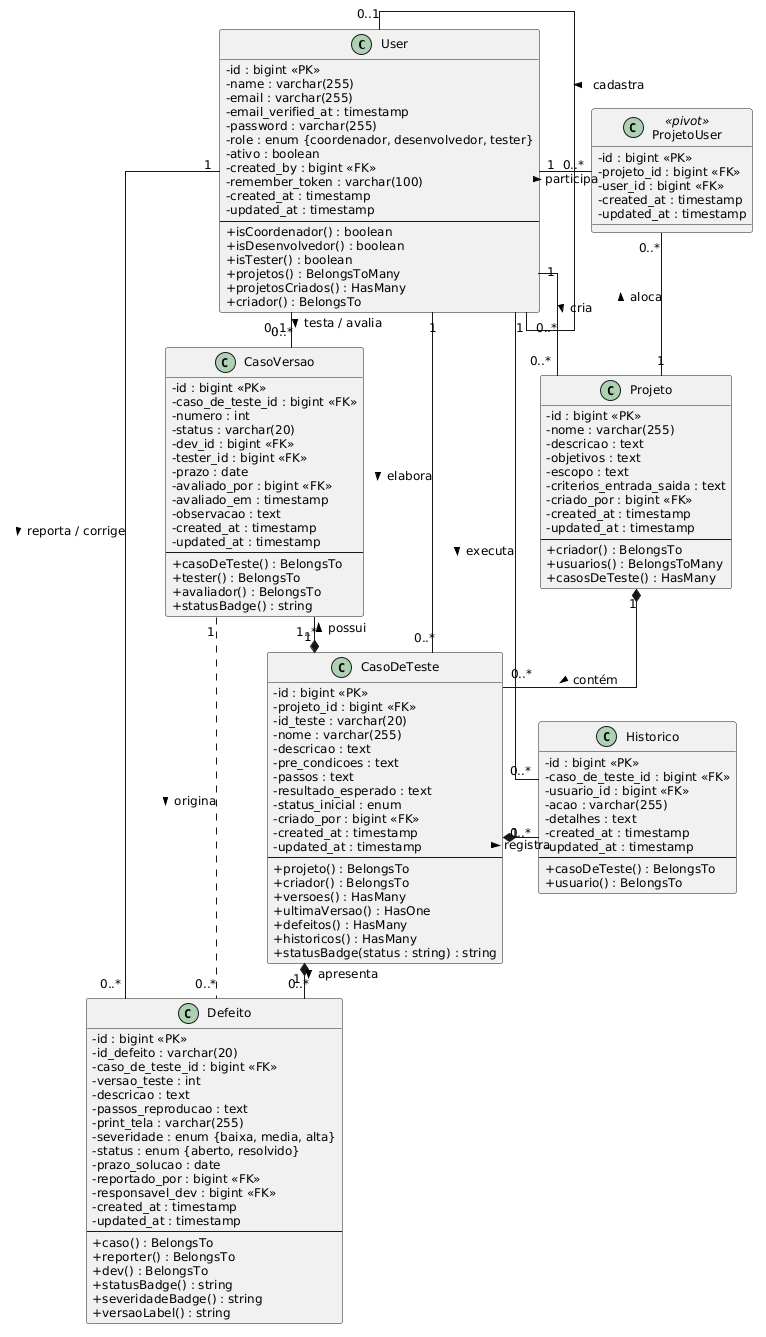
\includegraphics[width=1.0\textwidth, height=0.82\textheight, keepaspectratio]{./figuras/DiagramaDeClasse2.png} \\
    \vspace{0.15cm}
    {\raggedright \small Fonte: Elaborado pelo autor (2026).\par}
\end{figure}

\clearpage

\subsection{Modelo Lógico de Dados}

O armazenamento das informações orquestradas pelas classes do sistema exige uma infraestrutura relacional íntegra e normalizada. O Modelo Lógico do Banco de Dados, representado pelo Diagrama Entidade-Relacionamento (DER) na Figura \ref{fig:modelo_bd}, traduz a abstração orientada a objetos em tabelas físicas no SGBD MySQL, detalhando tipos de dados, chaves primárias (\texttt{PK}), chaves estrangeiras (\texttt{FK}) e restrições de integridade referencial.

No núcleo de domínio do banco de dados, a estrutura organiza-se em sete tabelas principais interligadas:
\begin{itemize}
    \item \textbf{\texttt{users}:} Armazena as credenciais de autenticação, o estado de ativação (\texttt{ativo}) e o papel de acesso (\texttt{role}) de cada usuário. Possui uma chave estrangeira auto-referenciada (\texttt{created\_by}) que aponta para o próprio \texttt{users(id)}, permitindo identificar o coordenador responsável pelo cadastro de cada membro;
    \item \textbf{\texttt{projetos} e \texttt{projeto\_user}:} A tabela \texttt{projetos} persiste os metadados de cada projeto de software (nome, descrição, objetivos, escopo e critérios de entrada/saída) e vincula seu autor via \texttt{criado\_por}. Como um projeto comporta múltiplos integrantes e um usuário pode atuar em diversos projetos, a tabela associativa \texttt{projeto\_user} resolve o relacionamento $N:N$ por meio das chaves estrangeiras \texttt{projeto\_id} e \texttt{user\_id};
    \item \textbf{\texttt{casos\_de\_teste}:} Registra a especificação base de cada roteiro de teste, incluindo o identificador amigável (\texttt{id\_teste}, como \texttt{CT-001}), pré-condições, passos de execução e resultado esperado, subordinando-se a um projeto (\texttt{projeto\_id}) e ao usuário autor (\texttt{criado\_por});
    \item \textbf{\texttt{caso\_versoes}:} Materializa o controle de versionamento dos testes (RF07). Em vez de sobrescrever o resultado de execuções anteriores, cada ciclo de avaliação gera uma linha vinculada a \texttt{caso\_de\_teste\_id}, contendo o número sequencial da versão (\texttt{numero}), o status (\texttt{pendente}, \texttt{aprovado} ou \texttt{reprovado}), o prazo limite, o avaliador designado (\texttt{tester\_id}) e os metadados de auditoria da execução (\texttt{avaliado\_por}, \texttt{avaliado\_em} e \texttt{observacao});
    \item \textbf{\texttt{defeitos}:} Centraliza os erros (\textit{bugs}) reportados durante a reprovação de um caso de teste. Além de vincular o caso de teste (\texttt{caso\_de\_teste\_id}) e o número da versão avaliada (\texttt{versao\_teste}), armazena o código identificador (\texttt{id\_defeito}, ex.: \texttt{DEF-001}), os passos para reprodução, o caminho da captura de tela (\texttt{print\_tela}), o nível de severidade (\texttt{baixa}, \texttt{media} ou \texttt{alta}), o status de resolução e as chaves estrangeiras que conectam o relator (\texttt{reportado\_por}) e o desenvolvedor encarregado da correção (\texttt{responsavel\_dev});
    \item \textbf{\texttt{historicos}:} Atua como uma trilha de auditoria imutável (RF13), registrando automaticamente cada evento relevante ocorrido no ciclo de vida de um caso de teste (\texttt{caso\_de\_teste\_id}), o autor da operação (\texttt{usuario\_id}), a descrição da ação (\texttt{acao}) e os detalhes da transição de estado (\texttt{detalhes}).
\end{itemize}

Complementarmente, o diagrama da Figura \ref{fig:modelo_bd} exibe à direita e nas extremidades as tabelas nativas de infraestrutura geradas pelas \textit{migrations} padrão do framework Laravel: \texttt{migrations} (controle de versão do esquema do banco), \texttt{sessions} e \texttt{password\_reset\_tokens} (gerenciamento de sessões ativas e recuperação de credenciais), \texttt{cache} e \texttt{cache\_locks} (otimização de consultas temporárias), bem como \texttt{jobs}, \texttt{job\_batches} e \texttt{failed\_jobs} (processamento de filas em segundo plano). O uso do mapeamento objeto-relacional (Eloquent ORM) atua como camada de abstração direta sobre o modelo físico representado na Figura \ref{fig:modelo_bd}, auxiliando na prevenção contra injeção de SQL e na manutenção da integridade dos dados.

\begin{figure}[!htb]
    \centering
    \caption{Modelo Lógico do Banco de Dados (DER) do Test-Manager.}
    \label{fig:modelo_bd}
    \vspace{0.2cm}
    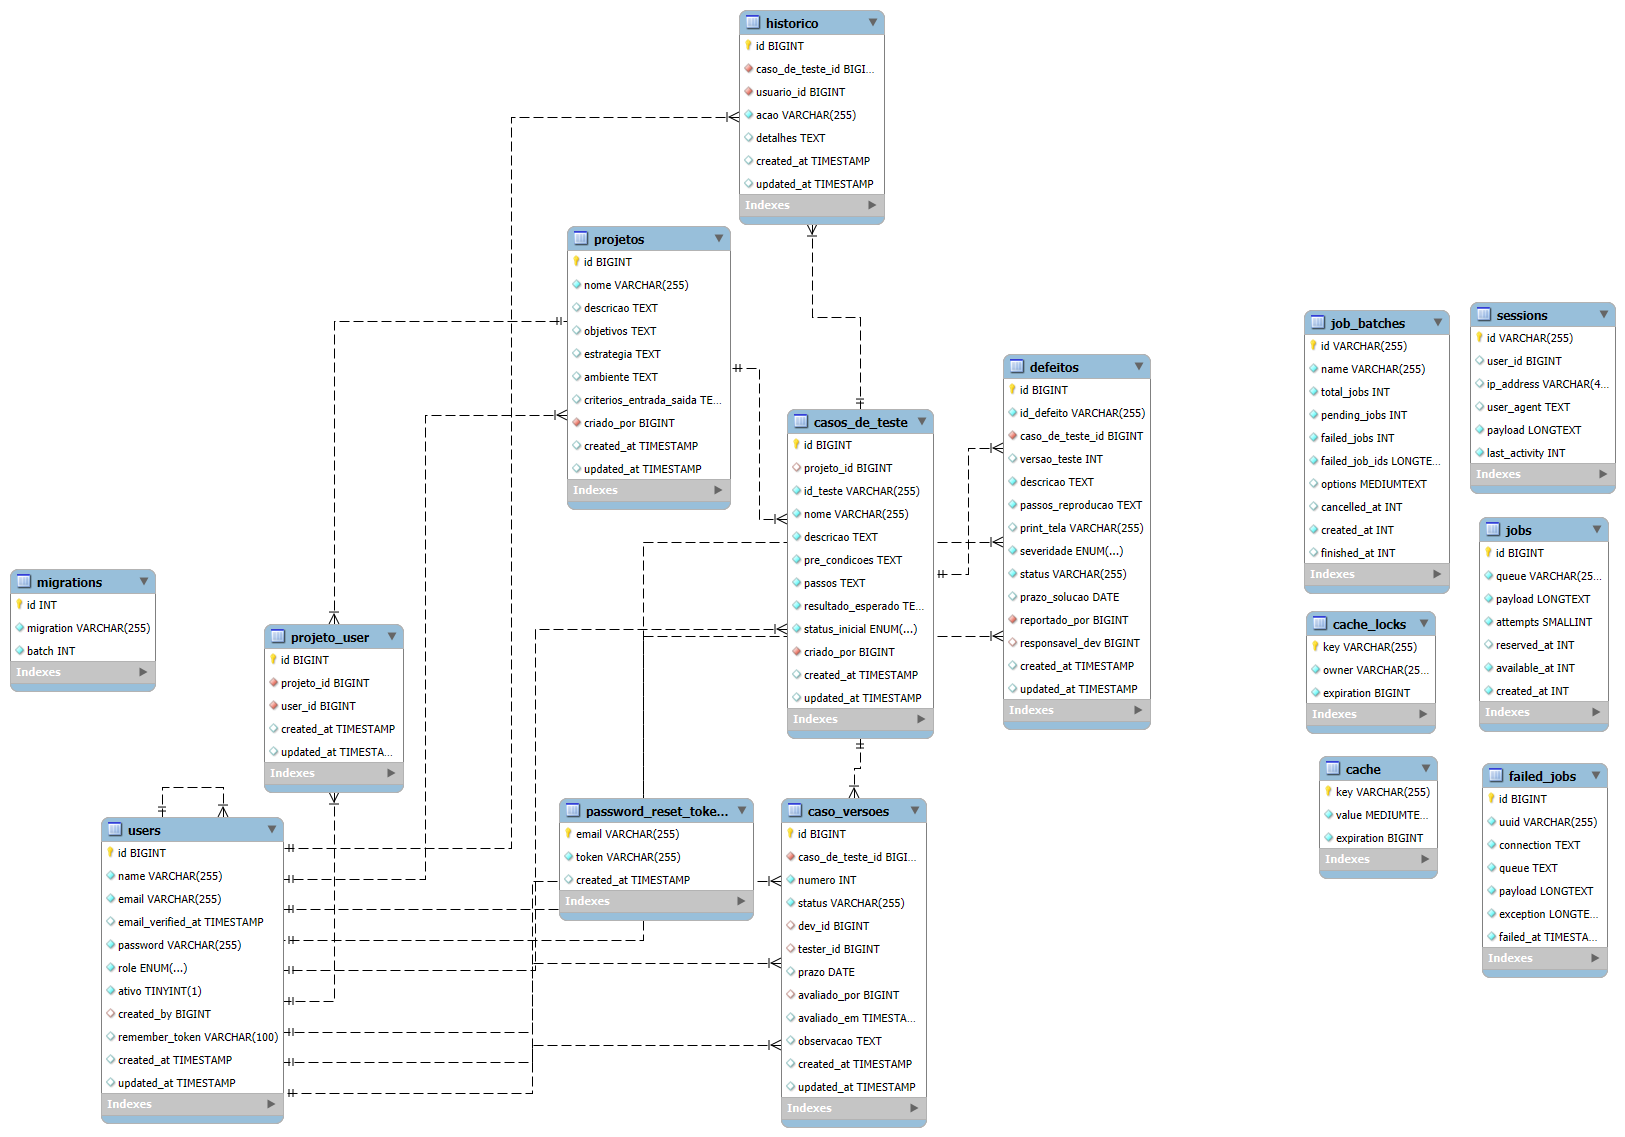
\includegraphics[width=0.98\textwidth, height=0.75\textheight, keepaspectratio]{./figuras/Modelobancodedados.png} \\
    \vspace{0.2cm}
    {\raggedright \small Fonte: Elaborado pelo autor (2026).\par}
\end{figure}